% !TeX spellcheck = de_DE
\documentclass{uebung_cs}
\usepackage{algo121}
\blattname{Wochenplan: Minimale Spannbaum}

%%%%%%%%%%%%%%%%%%%%%%%%%%%%%%%%%%%%%%%%%%%%%%%%%%%%%%%%%%%%%%%%%%%%%%%%%%%%

\newboolean{programming}
\setboolean{programming}{false}

%%%%%%%%%%%%%%%%%%%%%%%%%%%%%%%%%%%%%%%%%%%%%%%%%%%%%%%%%%%%%%%%%%%%%%%%%%%%

\begin{document}
\section*{Vorbereitung}
Lies E Kapitel 7 (oder CLRS Kapitel 23) und schau das Video der Woche.

\begin{figure}[h]
	\begin{center}
		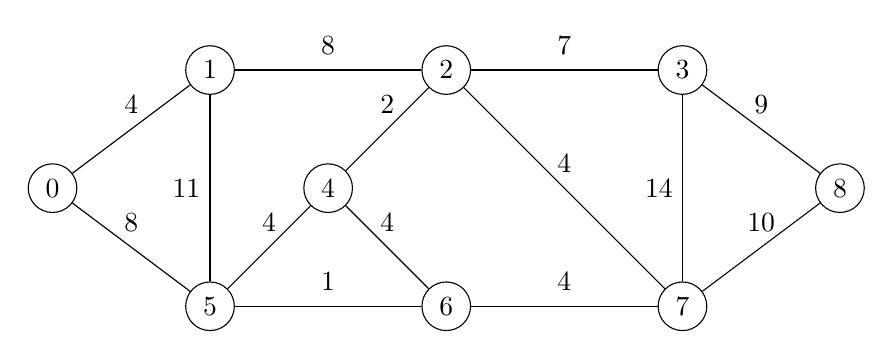
\begin{tikzpicture}
			\node[draw,circle] (v0) at (0,  1.5)	{$0$};
			\node[draw,circle] (v1) at (2,  3  )	{$1$};
			\node[draw,circle] (v2) at (5,  3  )	{$2$};
			\node[draw,circle] (v3) at (8,  3  )	{$3$};
			\node[draw,circle] (v4) at (3.5,1.5)	{$4$};
			\node[draw,circle] (v5) at (2,  0  )	{$5$};
			\node[draw,circle] (v6) at (5,  0  )	{$6$};
			\node[draw,circle] (v7) at (8,  0  )	{$7$};
			\node[draw,circle] (v8) at (10, 1.5)	{$8$};
			%
			\def\list {v0/v1/4, v0/v5/8, v1/v2/8, v2/v3/7, v2/v4/2, v2/v7/4, v3/v8/9, v4/v5/4, v4/v6/4, v5/v6/1, v6/v7/4, v7/v8/10}  % list elements
			\foreach \u\v\weight in \list
			{	\draw[-] (\u) -- (\v) node [midway, above=2pt] {\weight};
			}
			\def\vertical {v1/v5/11, v3/v7/14}  % list elements
			\foreach \u\v\weight in \vertical
			{	\draw[-] (\u) -- (\v) node [midway, left] {\weight};
			}
			
			%
		\end{tikzpicture}
		\caption{Graph für Aufgabe 1}
		\label{digraph}
	\end{center}
\end{figure}

\section*{Dienstag}
\begin{aufgabe}[Algorithmen und Eigenschaften]\label{tue-first}
	Gegeben sei der Graph G in Abbildung 1.
	\begin{enumerate}
		\item (\warmup) Führe den Kruskal Algorithmus manuell auf G aus.
		\item Führe den Prim Algorithmus manuell auf G aus (Startknoten 0). Zeige den Inhalt der Prioritätswarteschlange während der Ausführung.
		\item Zeige alle minimalen Spannbäume von G
		\item Gib einen effizienten Algorithmus zum finden eines Spannbaums an.
	\end{enumerate}
\end{aufgabe}

\begin{aufgabe}[Kabel für den Riedberg]
	Nach viel hin und her, sowie einigen Planungsfehlern, hat der Fachbereich 12 nun ganze N Gebäude (nummeriert $1,\ldots , N$) am Campus Riedberg.
	Top-Studentin Algolina hat die Verwantwortung dafür bekommen, dass alle Gebäude mit den neusten Lichtwellenkabeln verbunden sind.
	Zwei Gebäude $B_i$ und $B_j$ können für einen bestimmten Preis mit Lichtwellenkabeln verbunden werden.
	Algolina hat eine Liste mit M Preisen für das paarweise Verbinden zweier Gebäude (Gebäudepaare, die nicht in dieser Liste stehen, können nicht miteinander verbunden werden).
	Die Gebäude zählen als verbunden, wenn es einen Lichtwellenkabel-Weg zwischen allen Gebäude-Paaren gibt (es muss nicht unbedingt eine direkte Verbindung sein).
	Gegeben sei die Liste an Preisen.
	Entwirf einen Algorithmus, der Algolina dabei hilft, den günstigsten Gesamtpreis, bei dem alle Gebäude verbunden sind, zu berechnen.
	Du kannst annehmen, dass alle Gebäude verbunden werden können. 
\end{aufgabe}

\begin{aufgabe}[Graphen kappen]
	Zur Bestimmung eines minimalen Spannbaums wird folgender Algorithmus gegeben: Starte mit einem gewichteten, zusammenhängenden Graphen G. Betrachte die Kanten von G mit absteigendem Gewicht (vom höchstem zum niedrigsten Gewicht).
	Für jede Kante gilt: Behalte diese Kante, falls das Entfernen dieser Kante den Graphen in zwei Zusammenhangskomponenten aufteilen würde. Entferne sie falls dies nicht der Fall ist.
	Gib die finale Menge an Kanten zurück.
	\begin{enumerate}
		\item Führe den Algorithmus manuell auf G aus Abbildung 1 aus.
		\item Argumentiere, warum der Algorithmus den Minimalen Spannbaum von G findet.
	\end{enumerate}
\end{aufgabe}


\begin{aufgabe}[Eigenschaften von MSBs]
	Sei G ein gewichteter Graph.
	\begin{enumerate}
		\item Zeige, dass die Kante mit dem geringsten Gewicht in G immer im minimalen Spannbaum von G enthalten ist.
		Wie ist es mit der Kante mit dem höchsten Gewicht? 
		\item Wir skalieren alle Kanten-Gewichte in G indem wir sie mit einem Wert $c>0$ multiplizieren.
		Wie sieht der minimale Spannbaum für den neuen Graphen aus?
		\item Zeige, dass es einen einzigartigen minimalen Spannbaum für den Graphen G gibt, wenn alle Kanten-Gewichte verschieden sind.
		\textit{Hinweis:} erinnere dich an die Eigenschaften von minimalen Spannbäumen.
		\item Kruskals Algorithmus kann, abhängig davon, wie wir zwei Kanten mit gleichem Gewicht sortieren, verschiedene minimale Spannbäume für einen Graphen G zurückgeben.
		Zeige, dass für jeden minimalen Spannbaum T in G gilt, es gibt eine Möglichkeit die Kanten so zu sortieren, dass Kruskals Algorithmus T zurückgibt.
	\end{enumerate}
\end{aufgabe}


\begin{aufgabe}[Maximale Spannbäume]
	Gegeben sei ein gewichteter Graph G. Gib einen Algorithmus an, um einen maximalen Spannbaum von G zu bestimmen (also einen Spannbaum mit maximalem Gesamtgewicht).
	Hinweis: transformiere das Problem.
\end{aufgabe}


\begin{aufgabe}[MSBs und kleine Änderungen]
	Wir betrachten nun minimale Spannbäume auf Graphen deren Kantengewichte nicht paarweise verschieden sind.
	\begin{enumerate}
		\item Zeige, dass die Schnitt und Kreis Eigenschaften auch dann gelten, wenn die Kantengewichte nicht einzigartig sind (die Eigenschaften müssen entsprechend umformuliert werden).
		\item Schließe daraus, dass Prims und Kruskals Algorithmus auch in diesem Fall funktionieren.
	\end{enumerate}
\end{aufgabe}

\begin{aufgabe}[MSBs mit kleinen Kantengewichten, \hard]
	Sei G ein gewichteter Graph mit n Knoten und m Kanten so dass alle Kantengewichte Werte aus der Menge $\{ 1, 2, \ldots , 10\}$.
	Gib einen effizienten Algorithmus an, um einen minimalen Spannbaum von G zu bestimmen.
\end{aufgabe}


\end{document}
